\section{Theorie}
\label{sec:Theorie}

\subsection{Fehlerrechnung}

Für die Fehlerfortpflanzung bei Gleichungen mit $N$ fehlerbehafteten Größen
wird jeweils die Formel zur Gaußschen Fehlerfortpflanzung

\begin{equation*}
  \sigma = \sqrt{\sum_{i=1}^{N}\biggl(\frac{\partial f(x_{\g{i}})}{\partial x_{\g{i}}}
  \sigma_{\g{i}}\biggr)^2}
\end{equation*}
mit der jeweiligen Funktion $f(x_{\g{i}})$, den Messgrößen $x_{\g{i}}$ und den
zugehörigen Fehlern $\sigma_i$ verwendet.
Zur Berechnung des arithmetischen Mittels von $N$ Messwerten wird jeweils die
Formel

\begin{equation*}
  \bar{x} = \frac{1}{N}\sum_{i=1}^{N}x_{\g{i}}
\end{equation*}
mit den Messwerten $x_i$ benutzt.
Die Standardabweichung des Mittelwerts wird jeweils mit der Gleichung

\begin{equation*}
  \bar{\sigma} = \sqrt{\frac{1}{N-1}\sum_{i=1}^{N}(x_{\g{i}} - \bar{x})^2}
\end{equation*}
mit den $N$ Messwerten $x_i$ berechnet.


\subsection{Einleitung}

Der glühelektrische Effekt beinhaltet, dass beim Erhitzen einer Metalloberfläche
Elektronen emittiert werden. In diesem Versuch soll die Temperaturabhängigkeit
dieses Effekts untersucht und die damit verbundene Austrittsarbeit bestimmt
werden.

\subsection{Austrittsarbeit und Energieverteilung}

Aufgrund der meist sehr guten Leitfähigkeit von Metallen sind die Atome in
den Kristallgittern ionisiert und die Leitungselektronen bewegen sich
frei. Das Kristallgitter kann daher als konstanter Potentialtopf für die
Elektronen angenähert werden wie in Abbildung \ref{fig:TOPF} dargestellt.

\begin{figure}
  \centering
  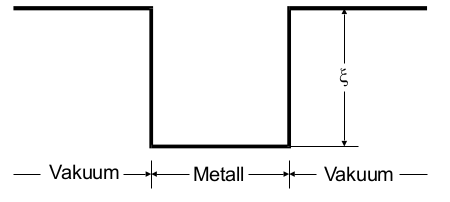
\includegraphics[height=3.5cm]{SommerAlbum15/PoTopf.png}
  \caption{Potentialtopf-Modell für ein Metall.\cite{anleitung}}
  \label{fig:TOPF}
\end{figure}

\FloatBarrier

Die Elektronen mit geringer kinetischer Energie
werden durch die positive Ladung im Topf festgehalten und nur solche mit
höherer kinetischer Energie als das Potential, also solche die die
Austrittsarbeit $e_0 Z$ leisten können, können dieses verlassen.
Aus dem Pauliverbot in der Quantenmechanik folgt, dass Elektronen, aufgrund
ihres halbzahligen Spins auch am absoluten Nullpunkt noch eine endliche
Energie besitzen. Die Maximalenergie $\zeta$ bei $T = \SI{0}{\kelvin}$ wird
Fermische Grenzenergie genannt. Sie hängt von der Elektronendichte im Metall ab.
Die Fermi-Diracsche Verteilungsfunktion
\begin{align}
  f(E) = \frac{1}{\symup{e}^{\frac{E-\zeta}{\symup{k}T}} + 1}
  \label{eqn:fermidirac}
\end{align}
beschreibt die Wahrscheinlichkeit, dass ein Zustand im thermischen
Gleichgewicht die Energie $E$ besitzt.
Sie ist in Abbildung \ref{fig:FermiDirac} skizziert.

\begin{figure}
  \centering
  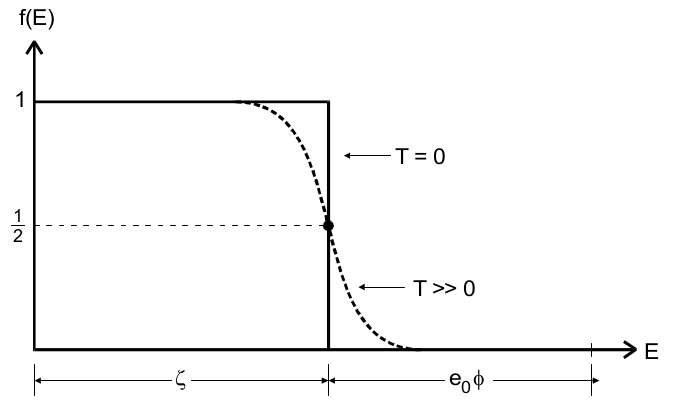
\includegraphics[height=7cm]{SommerAlbum15/FermiDirac.png}
  \caption{Skizze der Fermi-Dirac-Verteilung \eqref{eqn:fermidirac} bei
  $T = \SI{0}{\kelvin}$ und $T \gg \SI{0}{\kelvin}$.\cite{anleitung}}
  \label{fig:FermiDirac}
\end{figure}

\FloatBarrier

Da der Exponentialterm deutlich größer als eins ist, kann \ref{eqn:fermidirac}
zu
\begin{align}
  f(E) \approx \symup{e}^{\frac{\zeta-E}{\symup{k}T}}
  \label{eqn:fermidiracn}
\end{align}
genähert werden.

\subsection{Berechnung der Sättigungsstromdichte}

Aus der genäherten Fermi-Dirac-Gleichung kann die Sättigungstromdichte,
also die Anzahl an Elektronen, die pro Zeit durch ein Oberflächenelement
stoßen, in Abhängigkeit von der Temperatur bestimmt werden.
Dabei werden von den Elektronen in einem bestimmten Volumen nur solche
betrachtet, die die Ungleichung
\begin{align}
  \frac{p_\text{z}^2}{2\symup{m}_0} > \zeta + \symup{e}_0 \Phi,
\end{align}
mit dem Impuls $p_\text{z}$, der orthogonal auf der Oberfläche steht, und dem
Gitterpotential $\Phi$, erfüllen und damit energiereich genug sind um die
Oberfläche zu verlassen. Nach einigen Umformungen ergibt sich die
Richardson-Gleichung
\begin{align}
  j_\text{S}(T) = \frac{4\pi \symup{e}_0 \symup{m}_0 \symup{k}^2}{\text{h}^3} T^2
  \symup{e}^{\frac{-\symup{e}_0 \Phi}{\symup{k} T}}
  \label{eqn:richardson}
\end{align}
für die Sättigungsstromdichte.

\subsection{Hochvakuum-Diode}

Eine Skizze der Hochvakuum-Diode und ihrer Beschaltung ist in Abbildung
\ref{fig:hochvakuum} dargestellt.

\begin{figure}
  \centering
  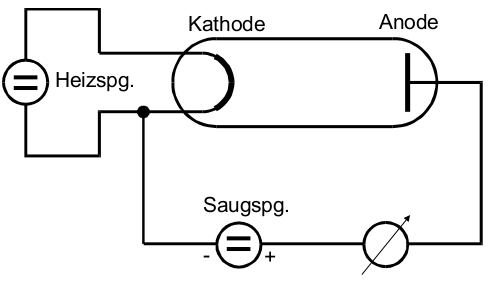
\includegraphics[height=4cm]{SommerAlbum15/Diode.png}
  \caption{Skizze einer Hochvakuum-Diode und ihrer Beschaltung.\cite{anleitung}}
  \label{fig:hochvakuum}
\end{figure}

\FloatBarrier

Anode und Kathode befinden sich in einem evakuierten Glasgefäß, damit
die emittierten Elektronen durch das erzeugte elektrische Feld direkt zur Anode
laufen und nicht mit Materie wechselwirken.
Durch den Heizstrom kann die Kathode auf $T = \SI{1000}{\kelvin}$ bis
$T = \SI{3000}{\kelvin}$ erhitzt werden.

\subsection{Raumladungsgleichung}

Bei niedrigen Betriebsspannungen der Diode hängt der gemessene Anodenstrom
von der Spannung ab, da das Feld nicht stark genug ist, um alle emittierten
Elektronen zur Anode zu beschleunigen.
Doch auch bei hohen Spannung, bevor der Sättigungsstrom erreicht wird,
sind Spannung und Strom nicht wie erwartet proportional.
Das lässt sich dadurch erklären, dass die zur Anode laufenden Elektronen
eine nicht vernachlässigbare Raumladungsdichte $\rho$ mit sich bringen,
sodass die neu emittierten Elektronen ein Gegenfeld spüren.
Aus der Kontinuitätsgleichung
\begin{align}
  j = -\rho v,
\end{align}
mit der Geschwindigkeit $v$ der Elektronen, und der Poisson- oder auch
Potential-Gleichung
\begin{align}
  \increment V = -\frac{\rho}{\symup{\epsilon}_0}
\end{align}
folgt nach einigen Rechnungen der Zusammenhang zwischen korrigiertem
Potential $V(x)$ und dem Abstand zur Kathode $x$
\begin{align}
  V^{\frac{3}{4}}(x) = \frac{3}{4}
  \sqrt{\frac{4 j}{\symup{\epsilon}_0\sqrt{2 \symup{e}_0 / \symup{m}_0}}}\cdot x.
\end{align}
Aus dieser Gleichung folgt, dass die Feldstärke $E$ proportional zu
$x^{\frac{1}{3}}$ und die Raumladung $\rho$ proportional zu $x^{-\frac{2}{3}}$
ist. Die Proportionalitäten sind in Abbildung \ref{fig:Ortsabh} skizziert.

\begin{figure}
  \centering
  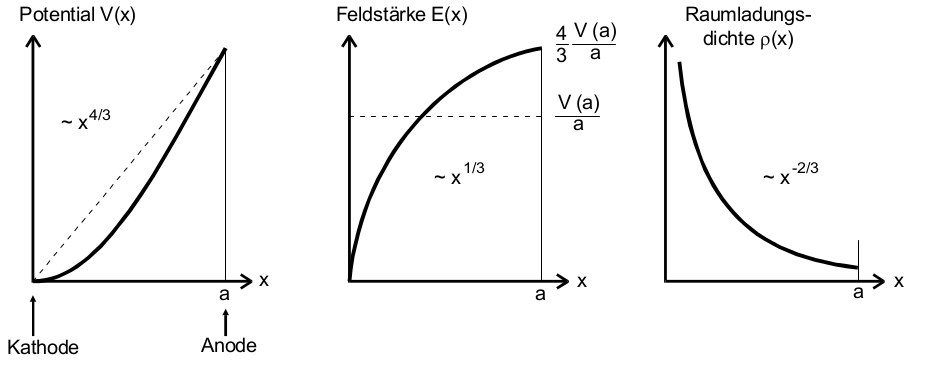
\includegraphics[height=6cm]{SommerAlbum15/Ortsabh.png}
  \caption{Proportionalität des Ortes zum Potentials $V(x)$, zur Feldstärke
  $E(x)$ und zur Raumladungsdichte $\rho(x)$ im Raumladungsgebiet einer
  Hochvakuum-Dioden-Kennlinie.\cite{anleitung}}
  \label{fig:Ortsabh}
\end{figure}

\FloatBarrier

Außerdem ergibt sich das Langmuir-Schottkysche Raumladungsgesetz an der
Anode bei $x = a$
\begin{align}
  j = \frac{4}{9} \symup{\epsilon}_0
  \sqrt{2 \symup{e}_0/\symup{m}_0} \frac{V^{\frac{3}{2}}}{a^2}.
  \label{eqn:LangSchott}
\end{align}

\subsection{Anlaufstromgebiet einer Hochvakuum-Diode}

Aus Gleichung \eqref{eqn:LangSchott} folgt, dass für $V=0$ die Stromdichte $j$
ebenfalls Null ist.
Da die Elektronen aber eine kinetische Eigenenergie besitzen, wird bei
einer Spannung $U=\SI{0}{\volt}$ oder sogar bei einer geringen Gegenspannung
noch ein Anodenstrom detektiert. Dieser Strom wird Anlaufstrom
genannt. In Abbildung \ref{fig:PotVer} sind die Potentialverhältnisse im
Anlaufstromgebiet dargestellt.

\begin{figure}
  \centering
  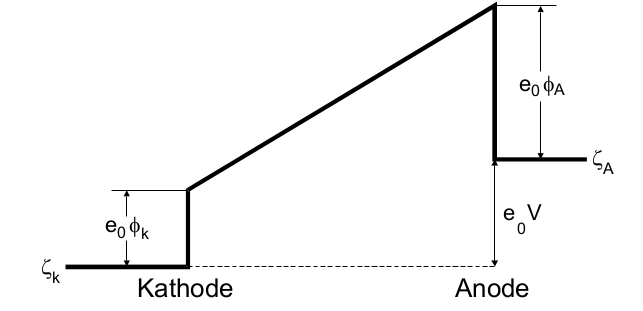
\includegraphics[height=4cm]{SommerAlbum15/PotVer.png}
  \caption{Potentialverhältnisse in einer Hochvakuum-Diode im
  Anlaufstromgebiet.\cite{anleitung}}
  \label{fig:PotVer}
\end{figure}

\FloatBarrier

Aus Abbildung \ref{fig:PotVer} ergibt sich die Anlaufstromdichte in Abhängigkeit
vom Potential
\begin{align}
  j(V) = j_0 \symup{e}^{-\frac{\symup{e}_0 \Phi_\text{A}+ \symup{e}_0 V}
  {\symup{k}T}},
  \label{eqn:Anlaufstromst}
\end{align}
wobei $\Phi_\text{A}$ die Austrittsarbeit des Anodenmaterials ist.

\subsection{Kennlinie einer Hochvakuum-Diode}

In Abbildung \ref{fig:Kennlinie} ist die Kennlinie einer Hochvakuum-Diode,
also der Zusammenhang zwischen der Spannung $U$ und Anodenstrom $I_\text{A}$,
skizziert.

\begin{figure}
  \centering
  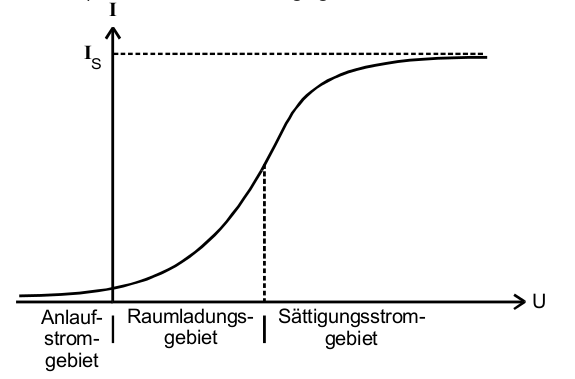
\includegraphics[height=6cm]{SommerAlbum15/Kennlinie.png}
  \caption{Skizze der Kennlinie einer Hochvakuum-Diode.\cite{anleitung}}
  \label{fig:Kennlinie}
\end{figure}

\FloatBarrier

Im Anlaufstromgebiet ist der Zusammenhang zwischen Spannung und Stromstärke
exponentiell. Im Raumladungsgebiet ist die Stromstärke proportional zu
$U^{\frac{3}{2}}$. Im letzten Bereich, dem Sättigungsstromgebiet, nähert
sich die Stromstärke mit steigender Spannung asymptotisch
einem Sättigunsstrom $I_\text{S}$ an.
